\documentclass[portrait,a0paper,fontscale=0.292]{baposter}

\usepackage[portuguese]{babel}
\usepackage[utf8]{inputenc}
\usepackage{graphicx}
\usepackage{helvet}
\renewcommand{\familydefault}{\sfdefault}

% Necessário para que o BibTeX funcione com o Baposter
% Esse arquivo precisa estar na mesma pasta do poster.tex
% Baixe em: 
% http://www.tex.ac.uk/tex-archive/biblio/bibtex/contrib/authordate/authordate1-4.sty
\usepackage{authordate1-4}

% The 'caption' package provides a nicer-looking replacement
\usepackage[labelfont=bf,textfont=it]{caption}

% Habilita subfigure.
\usepackage{subcaption}

% Habilita o uso de matrix.
\usepackage{amsmath}

% Habilita ambiente de algoritmos.
\usepackage[linesnumbered,portuguese]{algorithm2e}

% Divide igualmente o conteúdo da última página entre as duas colunas.
%\usepackage{flushend}

\usepackage{url}

% Copiado do template original:
\usepackage{relsize}
\usepackage{multirow}
\usepackage{booktabs}
\usepackage{multicol}
\usepackage{ae}

% Permite colocar direto o nome da imagem no includegraphics.
\graphicspath{{images/}}

% Distância entre colunas.
\setlength{\columnsep}{0.7em}

% Espessura da linha vertical que separa as colunas.
\setlength{\columnseprule}{0mm}


\begin{document}
\begin{poster}{
    grid=false,
    eyecatcher=false, % Exibe imagem à esquerda do título.
    colspacing=0.7em,
    %%% Definindo as cores das caixas. %%%
    headerColorOne=black!45!cyan!15,
    borderColor=black!45!cyan!15,
    %%% Estilo da borda. %%%
    textborder=faded,
    %%% Estilo da sub-caixa de título de cada caixa. %%%
    headerborder=open,
    headershape=roundedright,
    headershade=plain,
    background=none,
    bgColorOne=cyan!10!white,
    boxheaderheight=2.35em,
    %%% Espaço reservado para o título, autores e imagens superiores. %%%
    headerheight=0.153\textheight,
    %%% Número de colunas (de 1 a 6). %%%
    columns=2
}
% Imagem superior esquerda.
{
    %\parbox[t][5em][b]{7em}{
    %    \begin{tabular}{l}
    %        
\includegraphics[width=7em]{usp-logo}\\
    %        
\includegraphics[width=7em]{universidade}
    %    \end{tabular}
    %}
}
% Título do pôster.
{
    Identificando e classificando trechos de\\[0.2em]
    pistas no simulador de corridas TORCS
}
% Autores e nome da universidade.
{
    \\Vinícius K. Daros, Flávio S. C. da Silva\\[0.5em]
    Laboratório de Interatividade e Tecnologia de Entretenimento Digital
    \\[0.15em]
    Instituto de Matemática e Estatística - Universidade de São Paulo\\[0.5em]
    \texttt{\{vkdaros, fcs\}@ime.usp.br}
}
% Imagem superior direita.
{
    \parbox[t][5em][b]{7.5em}{
        \begin{tabular}{l}
            
\includegraphics[width=6em]{usp-logo}\\
            
\includegraphics[width=6em]{universidade}
        \end{tabular}
    }
    \parbox[t][7.2em][b]{4.5em}{
        
\includegraphics[height=5.75em]{logo-ime}
    }

    \parbox[t][7.45em][b]{8.75em}{
        
\includegraphics[height=6.1em]{sbgames_logo}
    }
}

\headerbox{Resumo}{name = abstract, column = 0, row = 0, span = 1}{
    Conhecer a forma da pista pode dar muitos benefícios à Inteligência
    Artificial que controla os carros nos jogos de corrida, mas esse tipo de
    informação nem sempre está disponível ao NPC. Tendo como plataforma de
    testes o simulador de corridas TORCS, mostramos neste trabalho um método
    capaz de construir um modelo de pista baseado apenas em leituras de um
    número limitado de sensores no carro de corrida. Também apresentamos uma
    técnica de segmentação do circuito indicando o início e fim de trechos
    distintos, classificando-os por suas características - como reta, curva
    suave, curva fechada, entre outros.
}

\headerbox{Construindo um modelo da pista}{name = model, column = 0,
                                           below = abstract}{
    \begin{multicols}{2}
        Durante uma volta de reconhecimento, o piloto virtual coleta dados
        através de sensores, como se fosse um robô. Ele tenta se manter no
        centro da pista, anda relativamente devagar (por volta de $60 Km/h$ em
        retas e $20 Km/h$ em curvas) e armazena a leitura dos sensores a cada 5
        metros. Ao fim da volta, os dados são processados. Assim, considerando
        pares consecutivos de medições, temos pequenos \textbf{segmentos} da
        pista, como visto na Figura \ref{fig:g-track-1_grid_cluster} ao lado.
%
%        \vskip 0.5em
%        Há outros trabalhos sobre formas de usar sensores para construir modelos
%        de pista. Por exemplo, \cite{quadflieg1} é apresentada uma técnica com
%        alta precisão. Porém são empregados vários sensores nessa tarefa, ao
%        contrário de nossa abordagem.

        \vskip 0.5em
        \begin{minipage}{0.48\textwidth}
            \centering
            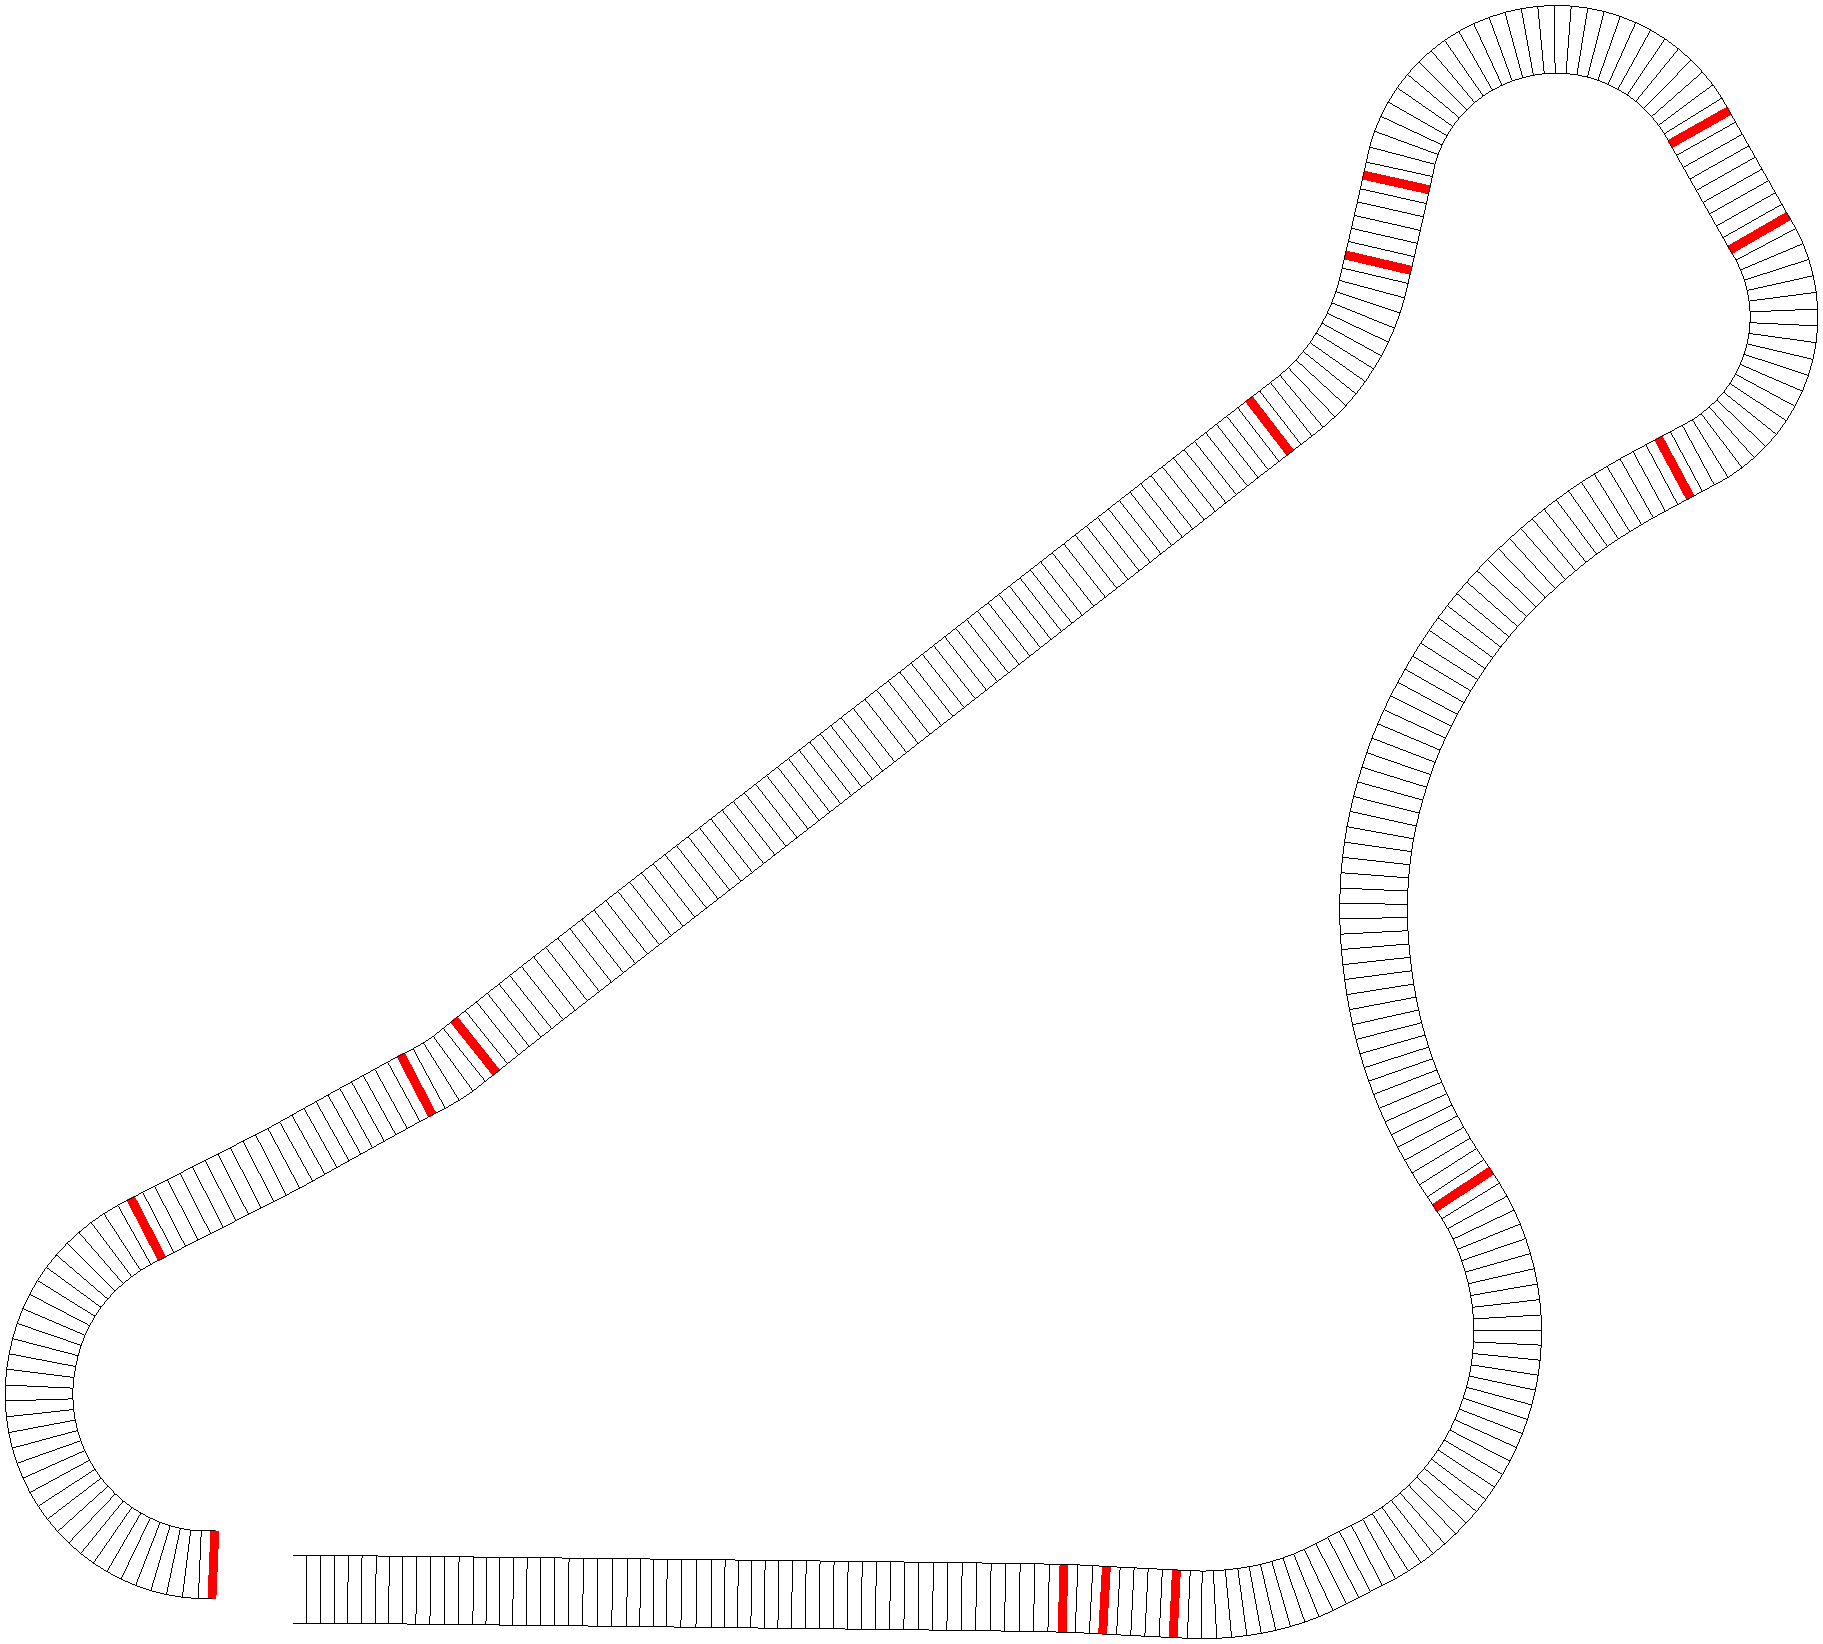
\includegraphics[width=0.8\textwidth]{g-track-1_grid_edge}
            \captionof{figure}{Pista \mbox{G-track-1} dividida em segmentos.
                               Traços vermelhos indicam os limites dos trechos.}
            \label{fig:g-track-1_grid_cluster}
        \end{minipage}
    \end{multicols}
}

\headerbox{Segmentação da pista}{name = segmentation, column = 0,
           below = model}{
    Agrupar os segmentos em \textbf{trechos} da pista é vantajoso por
    simplificar o modelo e a interpretação, além de facilitar o uso das
    informações. Porém para isso, é preciso descobrir se cada segmento faz parte
    de uma reta ou curva. Usando o sensor de quanto o volante estava virado no
    início e fim do segmento, conseguimos encontrar quanto o carro mudou de
    trajetória, ou seja, a \textbf{curvatura} do segmento.

    \vskip 1em
    Para realizar a segmentação, isto é, determinar os pontos nos quais um
    trecho termina e outro começa, nosso método avalia as variações das
    curvaturas como oscilações de um sinal e tenta identificar
    \textbf{patamares} que correspondem à regiões homogêneas na pista. Na Figura
    \ref{fig:g-track-1_plot}, a linha em vermelho ilustra o ``sinal'' referente
    à pista G-track-1 (Figuras \ref{fig:g-track-1_grid_cluster} e
    \ref{fig:g-track-1}).

    \begin{minipage}{\textwidth}
        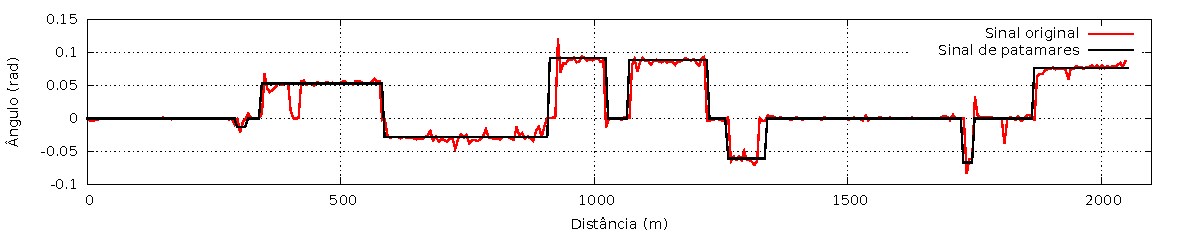
\includegraphics[width=\textwidth]{g-track-1_plot}
        \captionof{figure}{Curvatura de cada segmento da pista G-track-1 em
                           relação à distância do segmento até a linha de
                           largada.}
        \label{fig:g-track-1_plot}
    \end{minipage}
}

\headerbox{Algoritmo de segmentação}{name = algorithm, row = 0, column = 1}{
    %\vskip -0.8em
    \hfill
    \begin{minipage}{0.95\textwidth}
        \begin{algorithm}[H]
            \footnotesize
            \SetInd{0.5em}{0.6em}
            \SetKwFor{Para}{para}{faça}{fim}
            \SetKw{Return}{devolva}
            \SetAlgoNoLine

            \SetKwData{pontos}{ângulos}
            \SetKwData{dfs}{distâncias}
            \SetKwData{limiar}{limiar}
            \SetKwData{scale}{ESCALA}
            \SetKwData{base}{base}
            \SetKwData{flatD}{distFiltrada}
            \SetKwData{flatA}{angFiltrada}
            \SetKwData{bd}{distTrás}
            \SetKwData{ba}{angTrás}
            \SetKwData{fd}{distFrente}
            \SetKwData{fa}{angFrente}

            \SetKwFunction{Filtro}{FiltroDePatamar}
            \SetKwFunction{FiltroMedia}{FiltroDeMédia}
            \SetKwFunction{desvio}{DesvioPadrão}
            \SetKwFunction{push}{adiciona}
            \SetKwFunction{isGap}{éSalto}
            \SetKwFunction{isBaseline}{éPatamar}

            \Filtro{\dfs, \pontos, n}

            \Indp
                $\pontos \leftarrow \FiltroMedia{\pontos}$\\
                $\limiar \leftarrow \scale * \desvio{\pontos}$\\
                $\base \leftarrow 0$\\
                \flatD.\push{$0$}\\
                \flatA.\push{\base}\\
                \Para{$i \leftarrow 1$ \Ate $n - 2$}{
                    \Se{\isGap{\pontos$[i]$, \base, \limiar}}{
                        $\bd \leftarrow \dfs[i-1]$\\
                        $\fd \leftarrow \dfs[i]$\\
                        $\ba \leftarrow \base$\\

                        \Enqto{$i < n - 3$ \textbf{\emph e não} \isBaseline{\pontos, $i$}}{
                            $\triangleright$ \emph{Se houve mudança de sinal, ajusta a distância.}\\
                            \Se{$\pontos[i] * \pontos[i-1] <= 0$}{
                                $\bd \leftarrow \dfs[i-1]$\\
                                $\fd \leftarrow \dfs[i]$\\
                            }
                            $i \leftarrow i + 1$
                        }

                        $\fa \leftarrow \pontos[i]$\\
                        \Se{$|\fa| < MAX\_RETA$}{$\fa \leftarrow 0$}
                        $\triangleright$ \emph{Ponto do início do salto.}\\
                        \flatD.\push{\bd}\\
                        \flatA.\push{\ba}\\
                        $\triangleright$ \emph{Ponto do fim do salto.}\\
                        \flatD.\push{\fd}\\
                        \flatA.\push{\fa}\\
                        $\base \leftarrow \fa$\\
                    }
                }
                \flatD.\push{$\dfs[n]$}\\
                \flatA.\push{\base}\\
                \Return{\flatD, \flatA}
        \end{algorithm}
    \end{minipage}
}

\headerbox{Classificando os trechos}{name = classification, column = 1,
                                     below = algorithm}{
    \begin{multicols}{2}
        Depois da segmentação, cada trecho pode ser descrito por dois atributos:
        \emph(i) comprimento; \emph(ii) e raio, que determina o quanto uma curva é
        fechada. Como o comprimento de um trecho de curva está diretamente
        relacionado ao ângulo da mudança de direção do trajeto, optamos por usar
        esse ângulo para a classificação.

        \vskip 1em
        Nosso classificador agrupa trechos em 11 classes distintas. Embora não
        haja necessidade de rotular cada categoria, atribuímos a cada uma delas um
        nome de modo a facilitar a compreensão.

        \begin{minipage}{0.49\textwidth}
            \centering
            \vskip 0.25em
            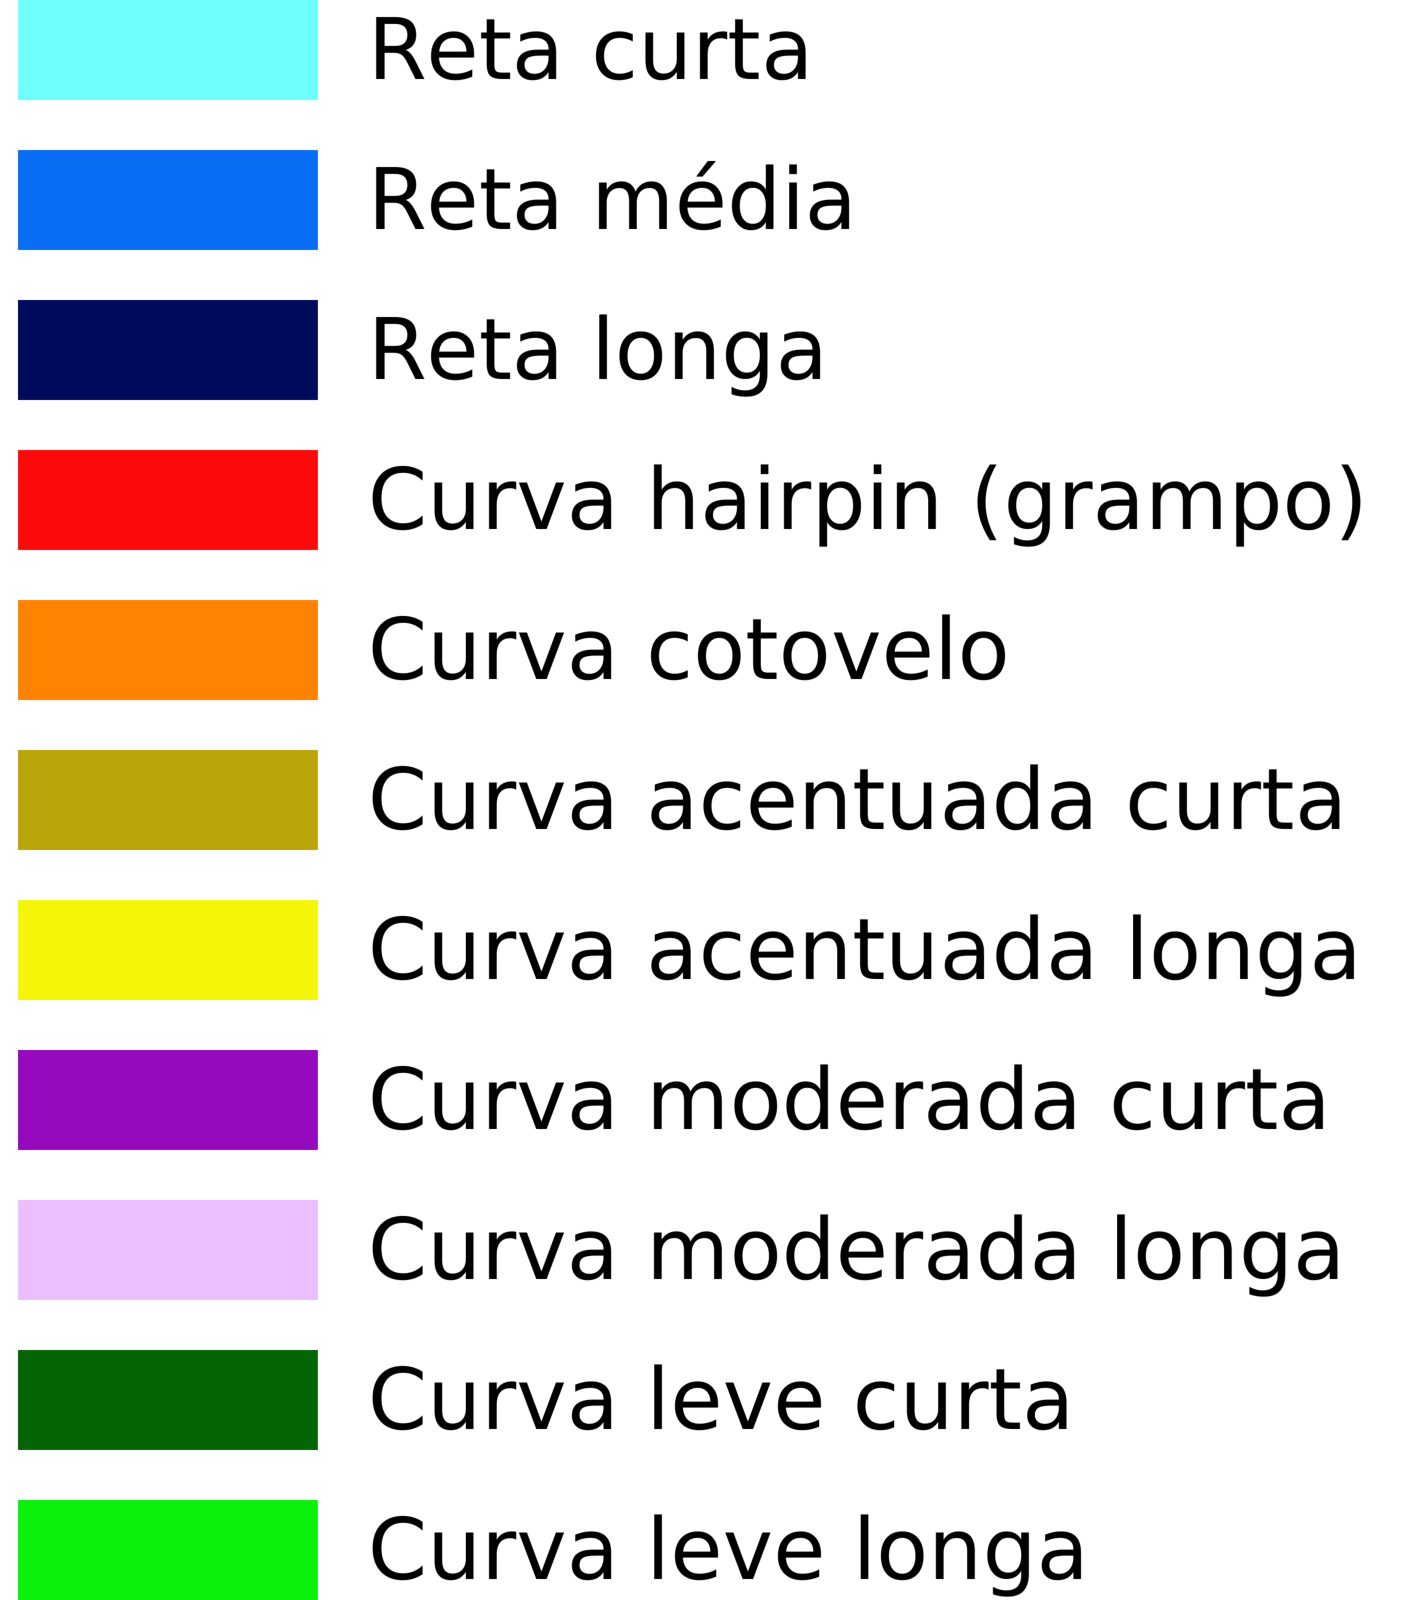
\includegraphics[width=0.97\textwidth]{legenda}
        \end{minipage}
    \end{multicols}
}

\headerbox{Resultados}{name = results, column = 0, below = segmentation,
                       span = 2}{
    Obtivemos resultados satisfatórios de segmentação e classificação nas 18
    pistas de asfalto que acompanham o \emph{TORCS}. Alguns exemplos estão na
    Figura \ref{fig:clusters}.

    \begin{minipage}{\textwidth}
        \vskip 1em
        \centering
        \begin{minipage}{0.18\textwidth}
            \centering
            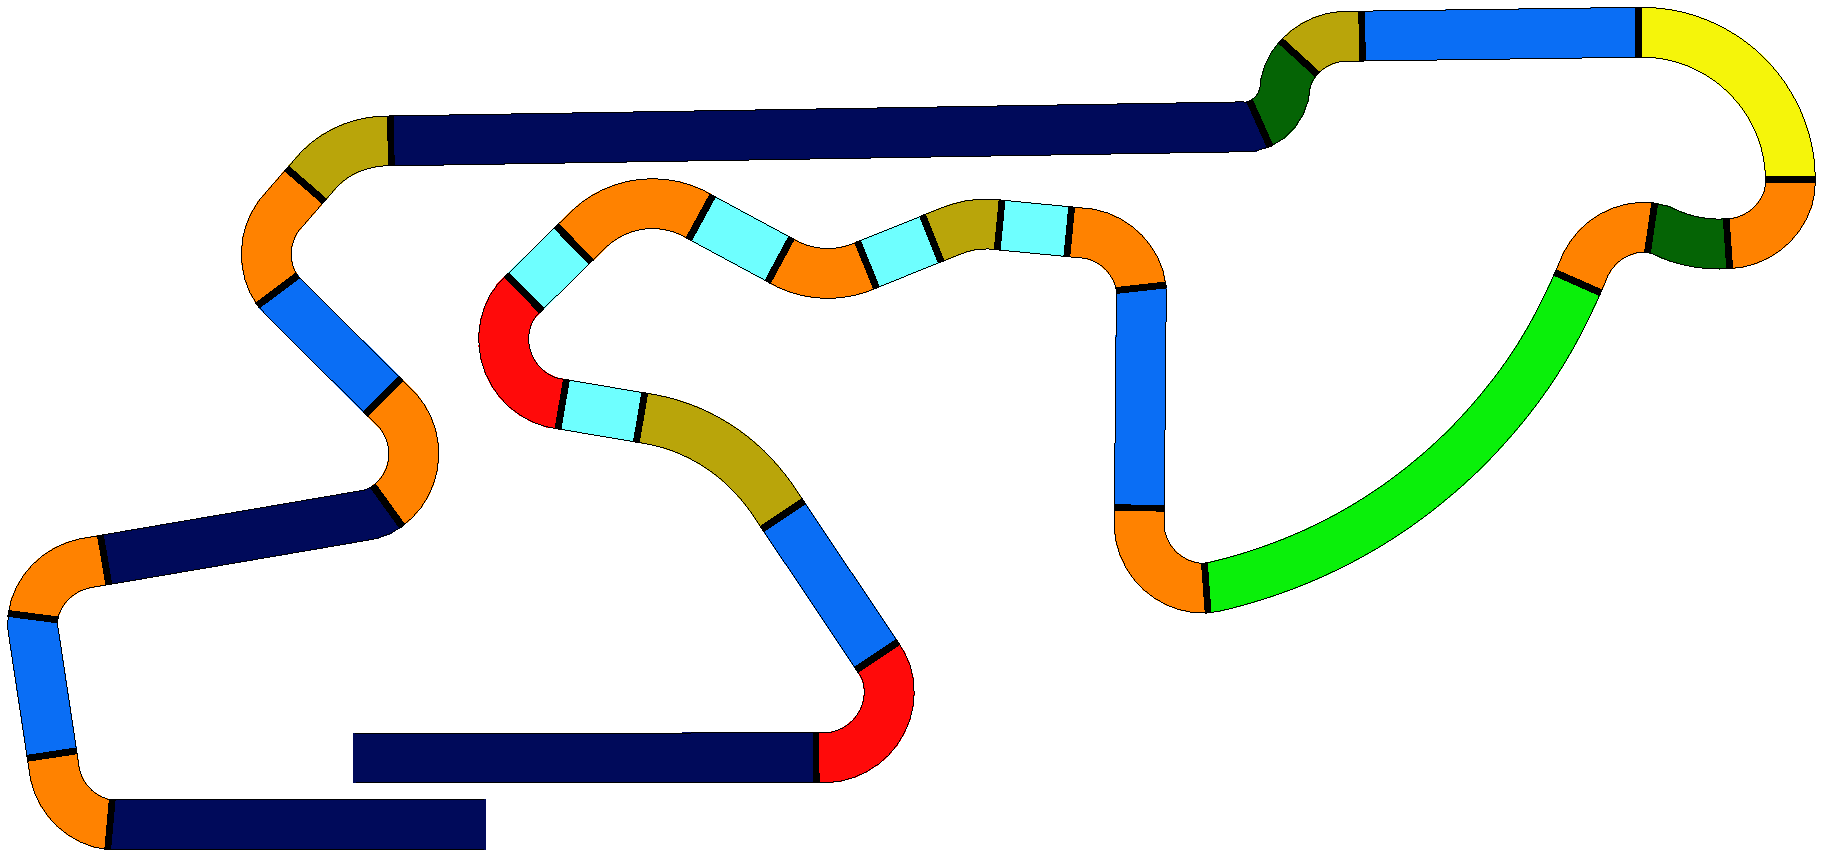
\includegraphics[width=\textwidth]{e-track-2}
            \captionof{subfigure}{E-track-2}
            \label{fig:e-track-2}
        \end{minipage}
        \begin{minipage}{0.24\textwidth}
            \centering
            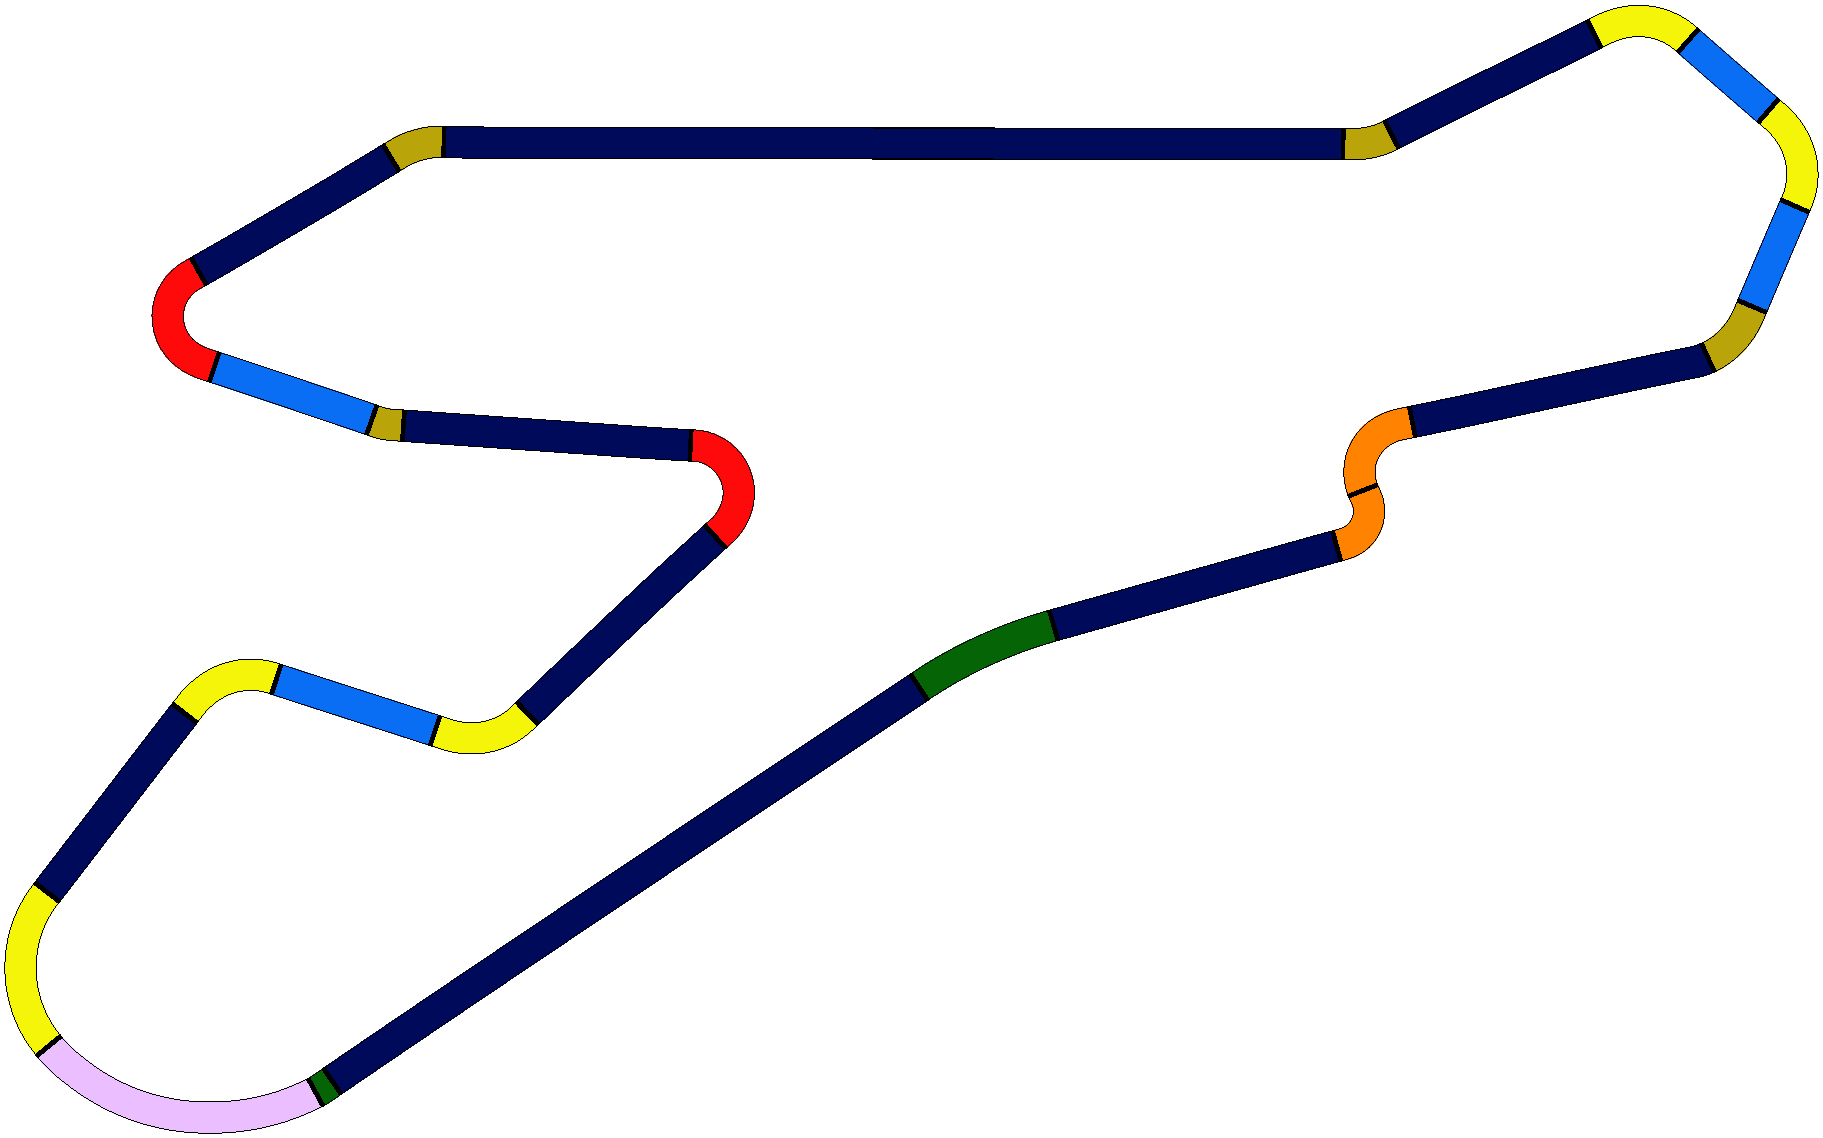
\includegraphics[width=\textwidth]{e-track-3}
            \captionof{subfigure}{E-track-3}
            \label{fig:e-track-3}
        \end{minipage}
        \hskip -0.02\textwidth
        \begin{minipage}{0.25\textwidth}
            \centering
            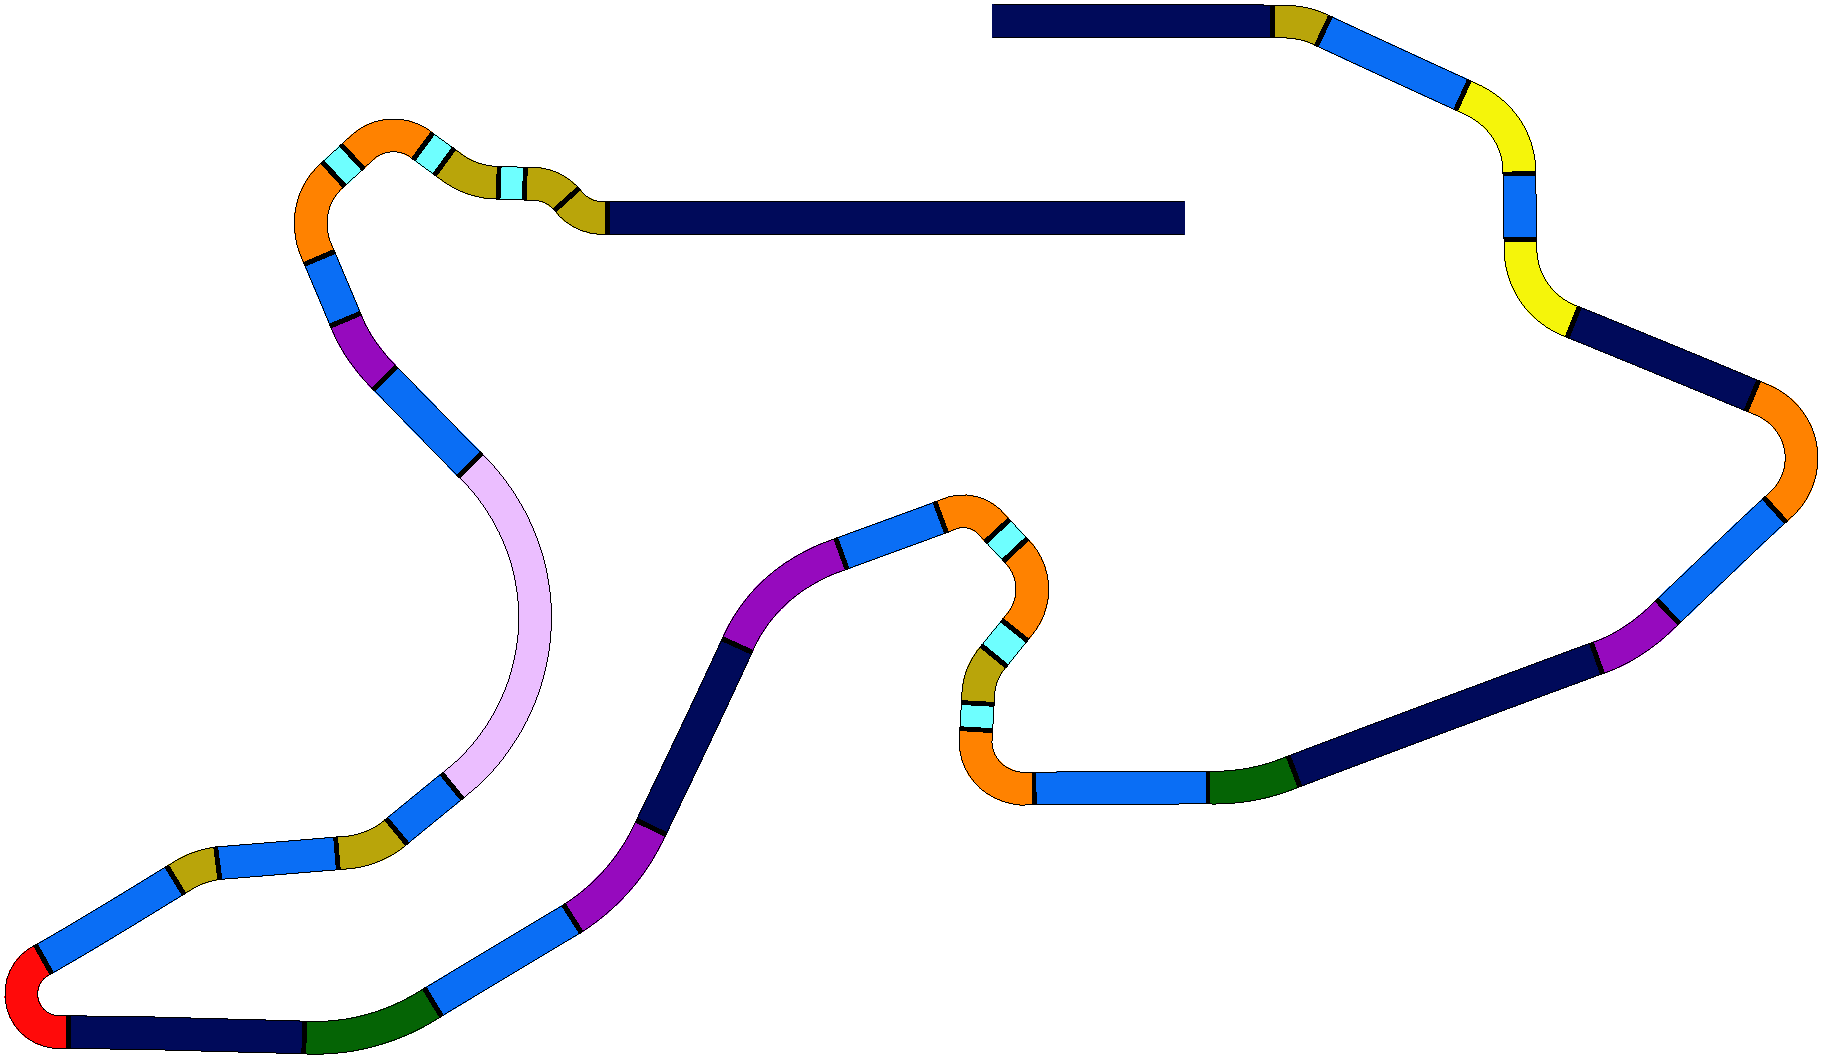
\includegraphics[width=\textwidth]{e-track-6}
            \captionof{subfigure}{E-track-6}
            \label{fig:e-track-6}
        \end{minipage}
        \begin{minipage}{0.15\textwidth}
            \centering
            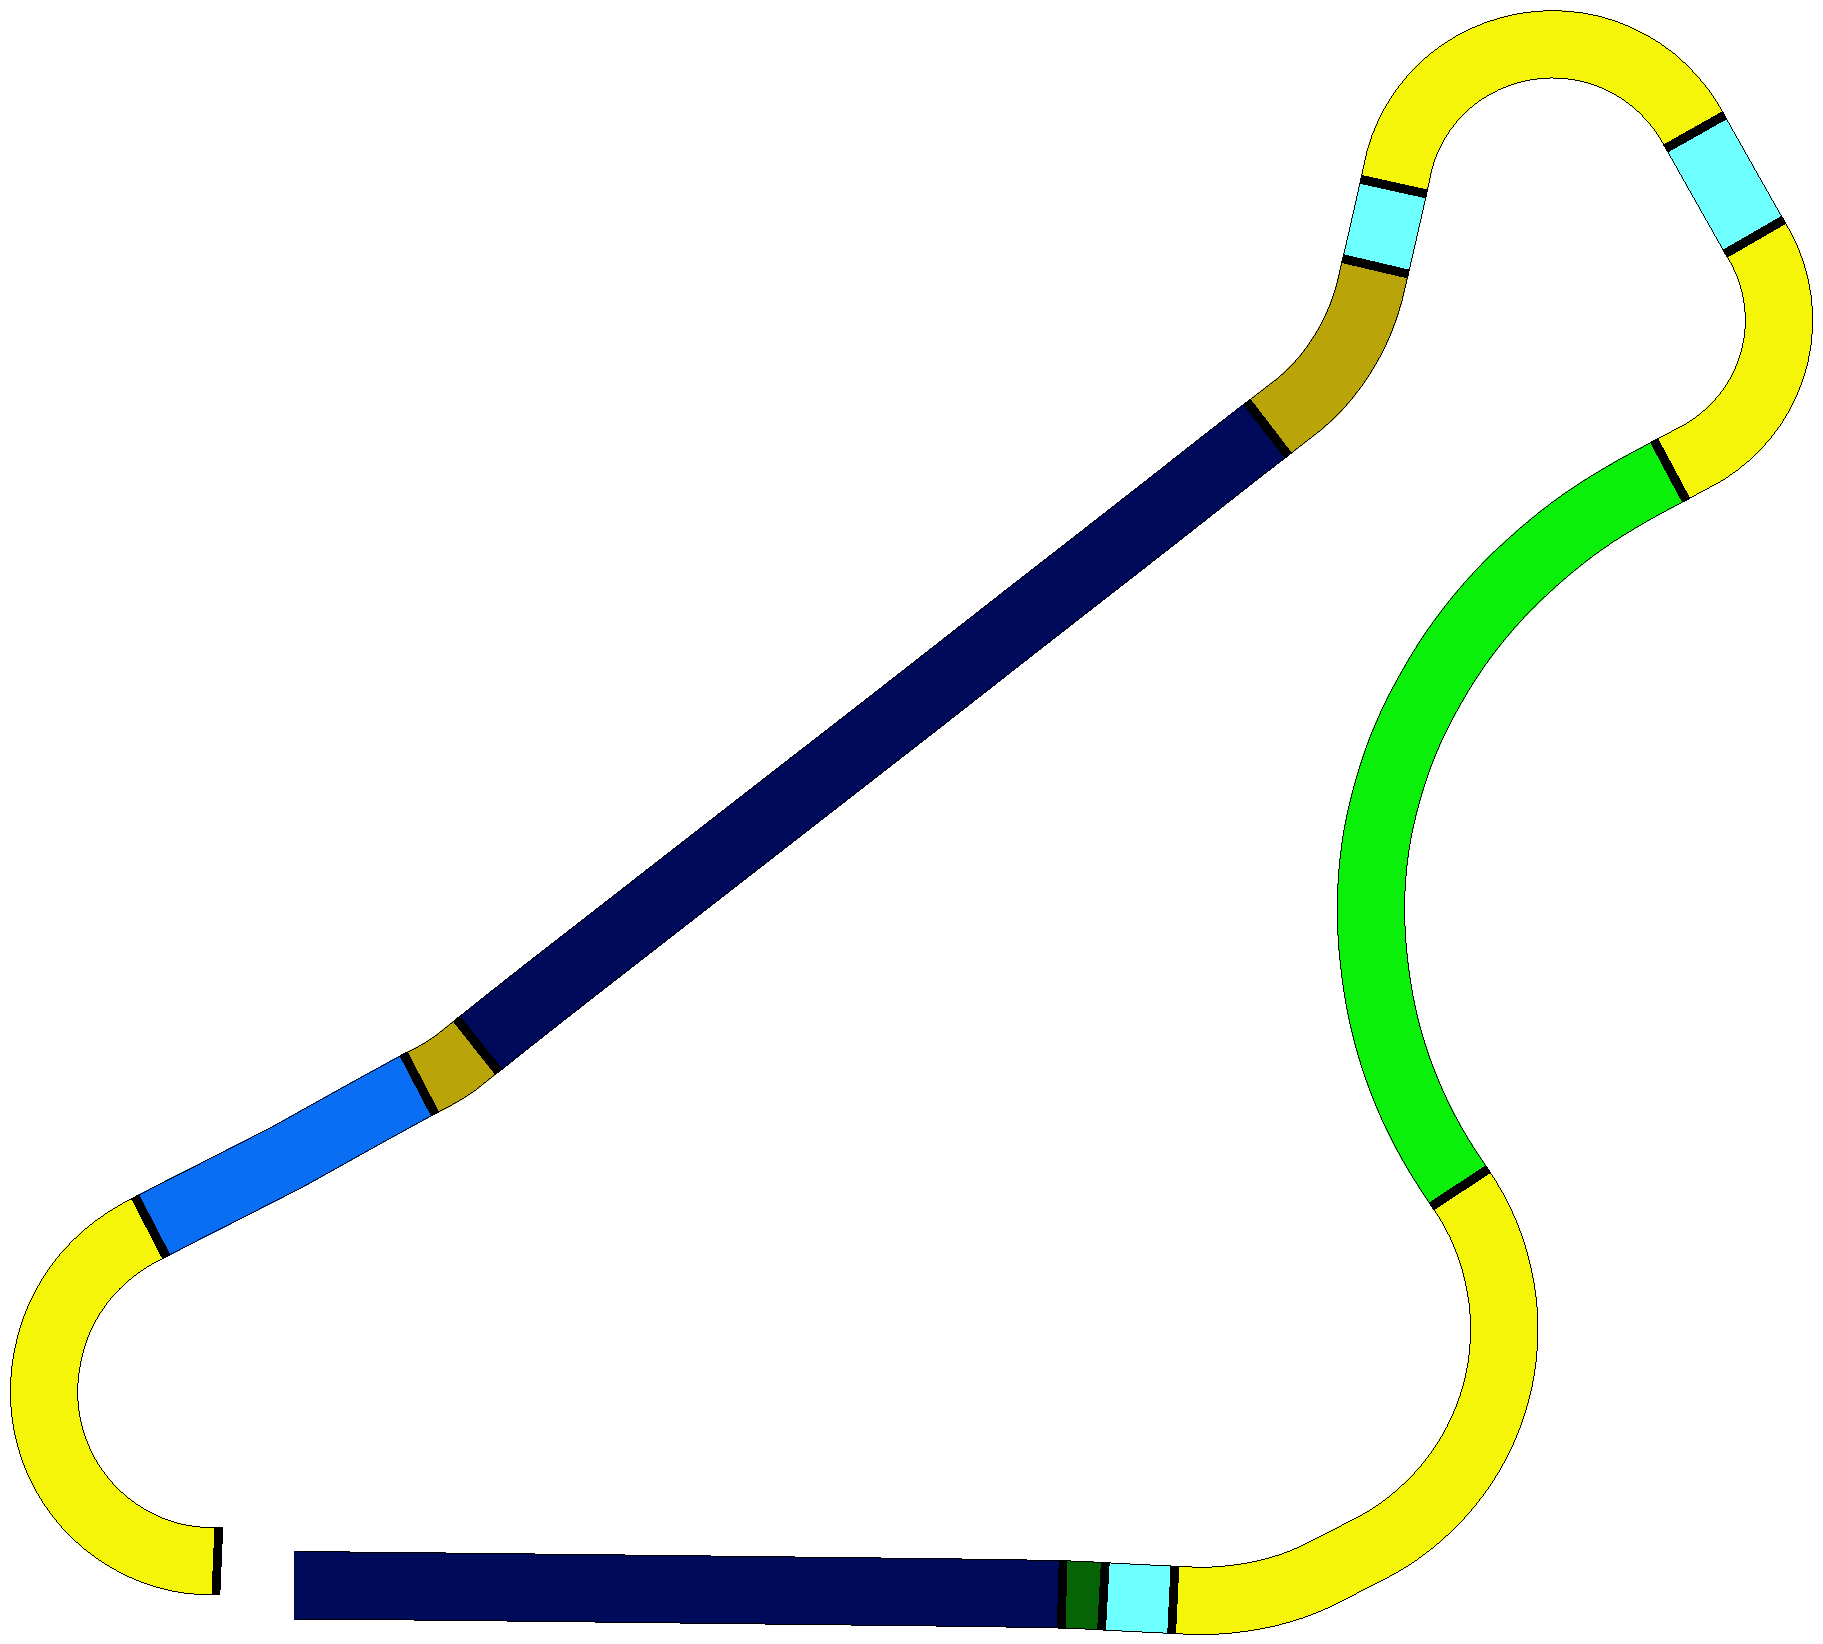
\includegraphics[width=\textwidth]{g-track-1}
            \captionof{subfigure}{G-track-1}
            \label{fig:g-track-1}
        \end{minipage}
        \hskip 0.02\textwidth
        \begin{minipage}{0.16\textwidth}
            \centering
            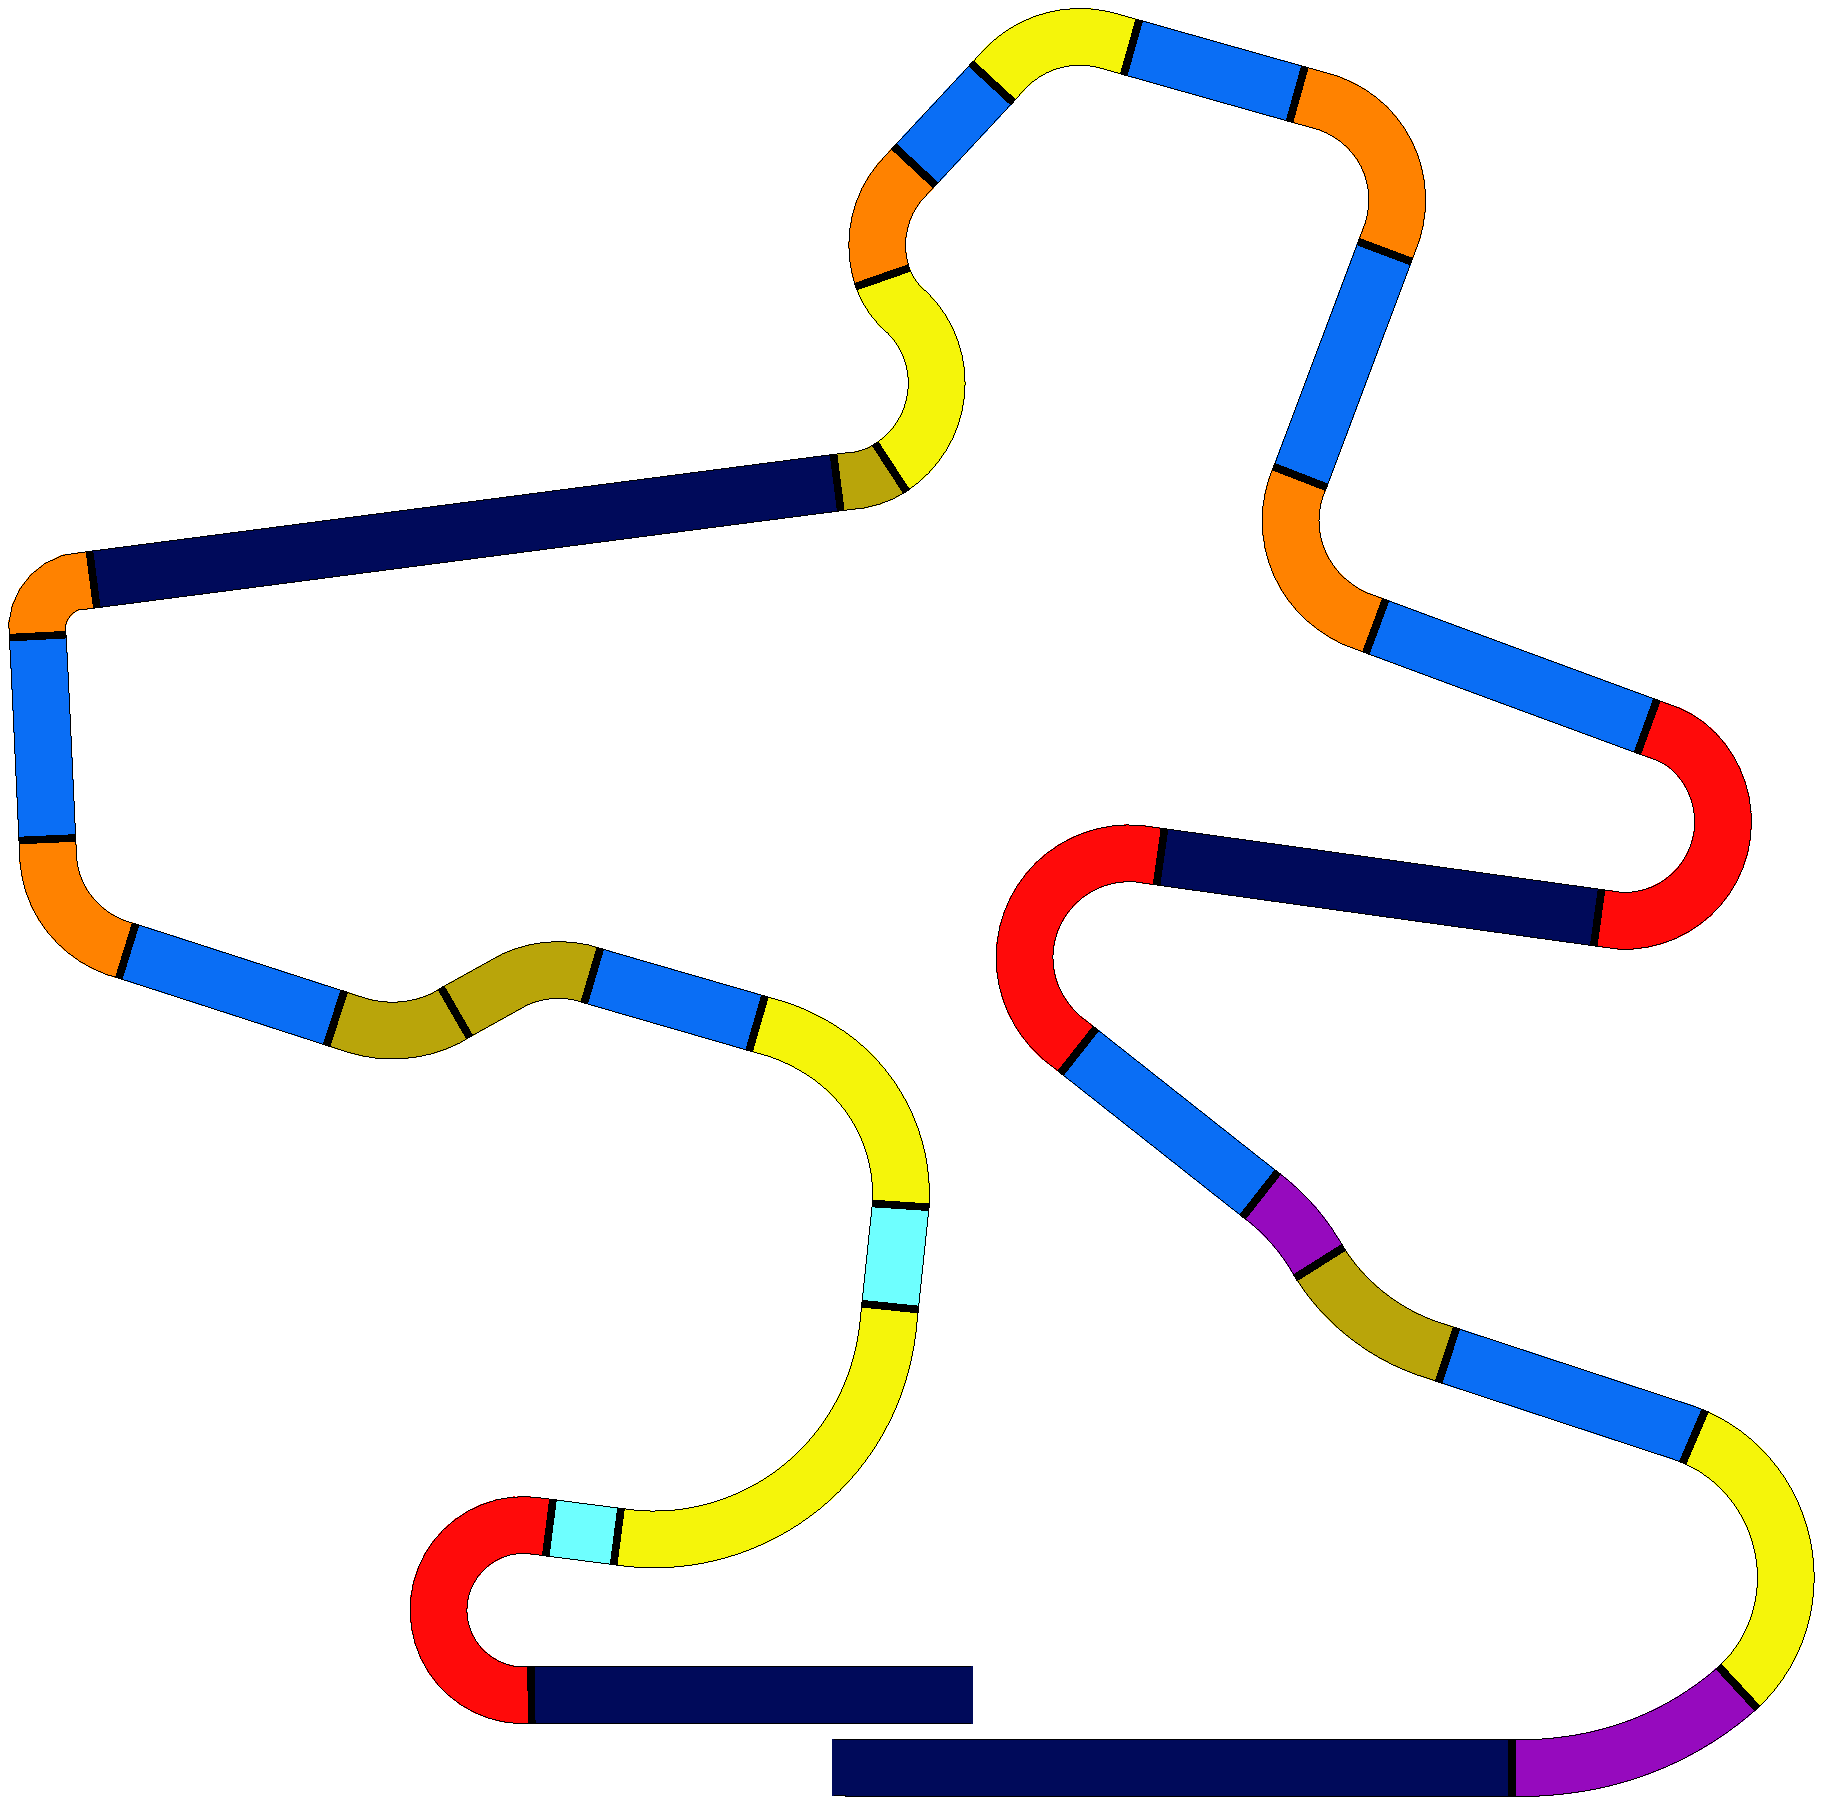
\includegraphics[width=\textwidth]{alpine-2}
            \captionof{subfigure}{Alpine-2}
            \label{fig:alpine-2}
        \end{minipage}
        \captionof{figure}{Exemplos de segmentação e classificação de pistas.}
        \label{fig:clusters}
    \end{minipage}
}

\end{poster}
\end{document}
